\documentclass{beamer}
\usepackage[size=a1,orientation=portrait,scale=1.4]{beamerposter}
\usetheme{LLT-poster}
\usecolortheme{ComingClean}

\usepackage[utf8]{inputenc}
\usepackage[T1]{fontenc}
\usepackage{libertine}
\usepackage[scaled=0.92]{inconsolata}
\usepackage[libertine]{newtxmath}

\author[mccardona@academia.usbbog.edu.co,jobeltran@academia.usbbog.edu.ccortes@academia.usbbog.edu.co]{Maria Camila Cardona,Jonathan Beltran,Camilo Cortes}
\title{Implementación de un sistema domótico enfocado en el ahorro energético}
\institute{Universidad de San Buenaventura}
\footimage{
\includegraphics[height=5cm]{12.jpg}}


\begin{document}
\begin{frame}[fragile]\centering

\begin{columns}[T]

%%%% First Column
\begin{column}{.48\linewidth}
\hspace{9em}
\begin{block}{Resumen}
En este proyecto de investigación, pretendemos corroborar información de productos domóticos que han brindado a la sociedad, estableciendo la relación que existe entre la solución mecatrónica con el ahorro energético dentro de un sistema eléctrico que estructura un hogar.
 También, observaremos que esta solución no implica de la acción de encender y apagar luces por una persona; básicamente lo que se explicará es la conexión entre un dispositivo central programable por el usuario, determinando cuándo hay flujo de corriente en la vivienda y cuando es necesario suspender este consumo. Además, este sistema le permitirá al usuario regular la energía en su casa generando un ahorro programado, donde el sistema estará conectado a los sensores distribuidos en la vivienda, con el fin de  identificar la presencia o ausencia de personas en cada espacio del hogar, logrando reducir el consumo de energía y disminuir los costos.
\end{block}

\begin{block}{Metodologia}
Para llevar acabo este proyecto debemos tener en cuenta los siguientes parámetros; principalmente debemos abordar una amplia investigación para recopilar información de como integrar sistemas de control energético en la estructura eléctrica de un hogar implementando domótica. Posteriormente, ingeniaremos una propuesta  y prototipo que se adapten a la idea generada, innovando las aplicaciones del área de la domótica.
\\ Diseñaremos el circuito integrado del hogar, el sistema de control y el regulador de energía eléctrico con el fin de reducir el alto consumo  eléctrico que normalmente se vive en los hogares. Ademas, evaluaremos el terreno y realizaremos el esquema arquitectónico  del hogar, para definir la ubicación y distribución de los elementos programables que establecen este sistema domótico, tales como sensores,temporizadores, etc.
\\Por medio de MASTER programaremos las fuente que recopila información para realizar acciones programadas del circuito eléctrico con ayuda de sistemas de control mixtos; Posteriormente implementaremos temporizadores que permiten controlar el encendido y apagado de luces, tomas-corrientes y tacos de luz. a dicha programación se le agregaran elementos como sensores, aparatos de cableado y termostatos con el fin de detectar la presencia y ausencia de individuos y reconocer en que momento se deben tener encendidas las luces teniendo en cuenta la distancia. 
\\Finalmente, proseguiremos a la instalación del regulador de energía y los objetos programables en el hogar y por medio de experimentación corroboraremos que este proyecto es eficaz generando ahorro energético
\end{block}


\end{column}

%%%% Second Column
\begin{column}{.47\textwidth}

\begin{block}{Introduccion}
ctualmente la humanidad se ha visto inmersa a la constante evolución tecnológica, donde se han presentando diversas soluciones con el fin de brindar una progresiva calidad de vida. Entre estas soluciones del campo tecnológico e ingenieril esta la domótica, que es definida por diferentes personas especializadas en este campo como la  'integración multímedia de los sistemas técnicos dentro del hogar'[1] asimismo, la Real Academia Española define la domótica como 'El conjunto de sistemas que automatizan las diferentes instalaciones de una vivienda [2] sin embargo, esta alternativa brinda un eficaz sistema para controlar el consumo de energía y agua ,el cual se hace por medio de lenguaje 'X10 y lonwords'[3], Representado matemática y físicamente por la ley de ohm; esta ley establece el circuito que integra un hogar,donde se relacionada la intensidad de corriente, diferencia de potencial y la resistencia,como lo muestra (Ecuacion 1)
\end{block}


\begin{center}
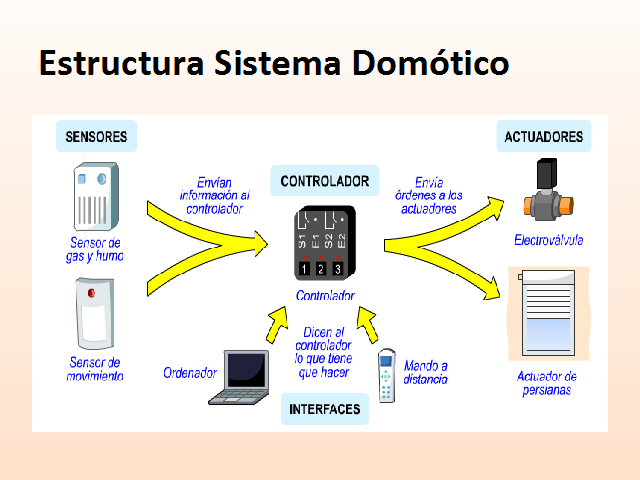
\includegraphics[width=.9\linewidth]{3.png}
\end{center}

\begin{block}{Ecuacion}
\begin{itemize}
\item Ley de ohm
\begin{align}
V &= I*R
\end{align}
\end{itemize}
\end{block}
\end{column}
\end{columns}





\vspace{0.2em}
\begin{block}{Objetivos General}
Diseñar un sistema de control que integre la estructura eléctrica que compone un hogar para ahorrar energía eléctrica.
\end{block}


\vspace{0.1em}
\begin{block}{Objetivos Especificos}
\begin{itemize}

\item Diseñar un regulador de energía eléctrica que permita consumir un rango moderado y establecido
\item Implementar temporizadores que permitan que las luces tengan un sistema de encendido y apagado en secuencias de tiempo.
\item Programar sensores de movimiento que detecten la presencia o ausencia de algún individuo para encender y apagar las luces automáticamente
\item Considerar las ventajas y desventajas que tiene llevar a cabo este proyecto.
\end{itemize}
\end{block}


\vspace{.2em}
\begin{block}{Referencias}
[1]A. Recuero, “Estado actual y perspectivas de la domótica,” Informes de la construcci´on, vol. 50, no. c, pp. 9–21, 1998 

[2] A. G. B. De Vela, M. J. S. Collado, and D. vasquez Junestrand Stefan, Xavier Passaret, “Domótica y hogar digital,” editorial paraninfo, vol. 27, no. 13, p. 228, 2005.

[3] L. F. Herrera Quintero, “Viviendas inteligentes ( Dom´otica ),” Revista Ingenier´ıa e investigaci´on, vol. 25, no. 2, pp. 47–53, 2005.

[4] J. Chaparro Mendivelso, “Dom´otica: la mutaci´on de la vivienda,” Vol.21, p. 136, 2003

[5]E. Sierra, A. Hossian, R. Garc´ıa-Mart´ınez, and P. Marino, Proceedings de la XI Reuni´on de Trabajo en Procesamiento de la Informaci´on y Control. Universidad Nacional de R´ıo Cuarto. P´ag, pp. 446–452, 2005

[6]C. Rojo Gallardo, “Proyecto De Instalaciones Para El Ahorro De Energ´ıa Y Agua En Una Vivienda Unifamiliar Situada En Sant Gregori (Girona),” algo, 2009.


\end{block}




\end{frame}
\end{document}